\documentclass[answers]{exam}
\renewcommand{\solutiontitle}{\noindent\textbf{}\par\noindent}

\usepackage{fullpage} % Package to use full page
\usepackage{parskip} % Package to tweak paragraph skipping
\usepackage{tikz} % Package for drawing
\usepackage{amsmath}
\usepackage{blindtext}
%\usepackage{hyperref}
\usepackage{graphicx}
\usepackage{enumerate}
\usepackage{caption}
\usepackage{subcaption}
\usepackage{multicol}
\usepackage{mathptmx}
\usepackage{amsmath}
\usepackage{amssymb}
\usepackage{nameref}
\usepackage{minted}
\usepackage{graphicx}

\newcommand{\mypoints}[1]{\textcolor{red}{(#1 points)}}
\newcommand{\achuta}[1]{\textcolor{magenta}{Achuta: #1}}
\newcommand{\chinmay}[1]{\textcolor{orange}{Chinmay: #1}}
\newcommand{\albert}[1]{\textcolor{purple}{Albert: #1}}
\newcommand{\myinput}[1]{\textcolor{blue}{#1}}

\title{\normalfont \normalsize
\textsc{{Department of Computer Science, UCLA \\
COM SCI 188: Computer Vision}}
\date{\vspace{-12ex}}
}
\begin{document}
\maketitle
\rule{\linewidth}{0.8pt} \\[6pt] 
\noindent
\large\textbf{\textsc{Instructor:}} Prof. Achuta Kadambi, Prof. Stefano Soatto \hfill \large\textbf{\textsc{Name:}} \myinput{Alexander Swerdlow}\\
\large\textbf{\textsc{TAs:}} Aditya Golatkar, Albert Zhao, Chinmay Talegaonkar \hfill 
\large\textbf{\textsc{UID:}} \myinput{305065891}
\rule{\linewidth}{0.8pt} \\[6pt] 

\begin{center}
{\textsc{Homework 2}} 
\end{center}
% \vspace{2cm}


\begin{table}[h]
\centering
\resizebox{0.8\textwidth}{!}{%
\begin{tabular}{cccc}
\hline
\multicolumn{1}{c}{\textsc{Problem}} &
\multicolumn{1}{c}{\textsc{Type}} &
\multicolumn{1}{c}{\textsc{Topic}} & \multicolumn{1}{c}{\textsc{Max. Points}} \\  \hline \\ 
 1 & Analytical & Filter Design &  10 \\ [2mm]
 2 & Analytical + Coding & Blob Detection &  10 \\ [2mm]
 3 & Coding & Corner Detection &  10 \\ [2mm]
 4 & Analytical & 2D Transformation &  10 \\ [2mm]
 5 & Analytical & Interview Question & 5 \\ [2mm]
\hline
\end{tabular}
}
\caption*{}
\label{}
\end{table}

\newpage

\section*{Motivation}

In the previous homework, we have seen how to process images using convolutions and mine images for features such as edges using image gradients. In this homework, we will detect other types of useful features in images such as blobs and corners that can be useful for a variety of computer vision tasks. We then transition from detecting useful features in images to relating different images via 2D transformations.

The problem set consists of: 
\begin{itemize}
    \item analytical questions to solidify the concepts covered in the class; and
    \item coding questions to implement some of the algorithms described in class using Python.
\end{itemize}

\section*{Homework Layout}
The homework consists of 5 problems in total, with subparts for each problem. There are 2 types of problems in this homework - analytical and coding. We encourage you to answer all the problems using the Overleaf document; however, handwritten solutions will also be accepted. 

\section*{Submission}

You will need to make two submissions: (1) Gradescope: You will submit a PDF with all the answers on Gradescope. (2) CCLE: You will submit your Jupyter notebook (.ipynb file) with filename $\{$your UID$\}$.ipynb with all the cells executed on CCLE. 


\newpage
\section{Filter Design \mypoints{10.0}}
In the class you were taught the Central Difference/Laplacian filter for detecting the edges in an image (by computing the gradients along the horizontal and vertical directions). In the discussion we derived those filters by approximating the first (for gradient) and second derivative (for Laplacian) of a univariate function $f(x)$ using the Taylor series expansion of $f(x+h)$ and $f(x-h)$, where $h$ is a small perturbation around $x$ with $h=1$ for the discrete case. These filters only consider the adjacent neighbours of the current pixel. In this question you will derive a high-order approximation for the two filters, such that the filters will use 2 adjacent neighbours. To summarize, you will be deriving a higher order approximation to the first/second derivative of $f(x)$. We will use $f^{(1)}(x),f^{(2)}(x)$ to denote the first and second derivative respectively.

\subsection{Compute $f(x+h)$ \mypoints{1.0}}
Write the Taylor series approximation for $f(x+h)$ around $f(x)$, such that the approximation error tends to 0 as $h^5$, i.e. consider only the first 5 terms in the Taylor series approximation. Use $f^{(1)}(x)$ for the first derivative, $f^{(2)}(x)$ for the second derivative and so on. 
\begin{solution} 
$
f(x+h)=f(x)+h f^{(1)}(x)+\frac{h^{2}}{2} f^{(2)}(x)+\frac{h^{3}}{3 !} f^{(3)}(x)+\frac{h^{4}}{4 !} f^{(4)}(x)+\mathcal O\left(h^{5}\right)
$
\end{solution}

\subsection{Compute $f(x-h)$ \mypoints{1.0}}
Similarly, write the Taylor series approximation for $f(x-h)$ around $f(x)$, such that the approximation error tends to 0 as $h^5$.
\begin{solution}
$
f(x-h)=f(x)-h f^{(1)}(x)+\frac{h^{2}}{2} f^{(2)}(x)-\frac{h^{3}}{3 !} f^{(3)}(x)+\frac{h^{4}}{4 !} f^{(4)}(x)-\mathcal O\left(h^{5}\right)
$
\end{solution}

\subsection{Compute $f(x+h)-f(x-h)$ \mypoints{1.0}}
\label{difference}
Using the expressions you obtained in the previous two parts, compute the expression for $f(x+h)-f(x-h)$. You may assume that $\mathcal{O}(h^5)$ tends to 0, so that you can neglect the term. You will be using this result to compute a high-order approximation to $f^{1}(x)$.
\begin{solution}
$
f(x+h)-f(x-h)=2 h f^{(1)}(x)+\frac{2h^{3}}{3} f^{(3)}(x)
$
\end{solution}

\subsection{Unknowns at each pixel \mypoints{1.0}}
\label{unknowns}
Let's assume that you have access to $f(x)$, which is a 1D signal (or equivalently one row in an image). This means that you can easily obtain the values for $f(x)$, $f(x \pm h)$, $f(x \pm 2h)$ and so on (assuming appropriate zero padding for start and end values). However, for each pixel $x$, if you only consider using its adjacent neighbours ($\pm h$), then the equation in the previous part has 2 unknowns. What are the two unknowns?
\textit{Note:} $h=1$ for the discrete case, so $h$ is not an unknown. But don't substitute $h=1$ as of now; we will substitute it later.
\begin{solution}
The two unknowns are $f^{(1)}(x)$ and $f^{(3)}(x)$
\end{solution}

\subsection{Compute $f^{(1)}(x)$ \mypoints{1.0}}
\label{gradient}
From the previous part, you know that for each pixel $x$, if we only consider $x \pm h$, then we have 1 equation and 2 variables (underdetermined system). To mitigate this issue, we consider two adjacent neighbours for each pixel ($x \pm 2h$) in addition to $x \pm h$. Replace $h$ with $2h$ in the previous equation and you will get another equation for that pixel. So now, for each pixel, you have 2 equations and 2 variables. One equation should have $f(x \pm h)$ and the other should have $f(x \pm 2h)$. Using these two equations, solve for $f^{(1)}(x)$.
\begin{solution}
$
f(x+h)-f(x-h)=2 h f^{(1)}(x)+\frac{2h^{3}}{3} f^{(3)}(x) \\
f(x+2h)-f(x-2h)=4 h f^{(1)}(x)+\frac{16h^{3}}{3} f^{(3)}(x) \\\\
f^{(1)}(x) = \frac{8f(x+h)-8f(x-h)-f(x+2h)+f(x-2h)}{12 h}
$
\end{solution}

\subsection{Convolution Kernel \mypoints{1.0}}
What is the convolution kernel corresponding to the new filter for $f^{(1)}(x)$? Substitute $h=1$ for the discrete case. This filter is now a higher order central-difference filter which can be used to compute the gradients/edges.
\begin{solution}
$
f_x = \begin{pmatrix}
\frac{1}{12} & \frac{-2}{3} & 0 & \frac{2}{3} & \frac{-1}{12}
\end{pmatrix}
$
\end{solution}

\subsection{Laplacian Filter \mypoints{1.0}}
We will repeat the same exercise as the previous parts; however, now we compute a higher order approximation to the Laplacian filter. Similar to \ref{difference}, compute the expression for $f(x+h) + f(x-h)$.
\begin{solution}
$
f(x+h)+f(x-h)=2f(x) + h^2 f^{(2)}(x)+\frac{2h^{4}}{4!} f^{(4)}(x)
$
\end{solution}

\subsection{Unknowns for the Laplacian \mypoints{1.0}}
Similar to \ref{unknowns}, what are the two unknowns for each pixel in the expression from the previous part?
\begin{solution}
The two unknowns are $f^{(2)}(x)$ and $f^{(4)}(x)$
\end{solution}

\subsection{Compute $f^{(2)}(x)$ \mypoints{1.0}}
Similar  to \ref{gradient}, use $f(x \pm 2h)$ to solve for $f^{(2)}(x)$. Write the expression for $f^{(2)}(x)$.
\begin{solution}
$
f(x+h)+f(x-h)=2f(x) + h^2 f^{(2)}(x)+\frac{2h^{4}}{4!} f^{(4)}(x) \\
f(x+2h)+(x-2h)=2f(x) + 4h^2 f^{(2)}(x)+\frac{32h^{4}}{4!} f^{(4)}(x) \\\\
f^{(2)}(x) = \frac{16f(x+h)+16f(x-h)-f(x+2h)-f(x-2h)-30f(x)}{12h^2}
$
\end{solution}

\subsection{Convolution Kernel \mypoints{1.0}}
What is the corresponding convolution for the filter you derived in the previous part? Use $h=1$ for the discrete case.
\begin{solution}
$
f_{xx} = \begin{pmatrix}
\frac{-1}{12} & \frac{4}{3} & \frac{-5}{2} & \frac{4}{3} & \frac{-1}{12}
\end{pmatrix}
$
\end{solution}

\newpage
\section{Blob Detection \mypoints{10.0}}
In this question, you will be using the Laplacian of Gaussian (LoG) filter to detect blobs in an image. Let's consider a 2D Gaussian $G_{\sigma}(x,y) = \dfrac{1}{2\pi \sigma^2} e^{-\big(\dfrac{x^2+y^2}{2\sigma^2}\big)}$. Remember that we need to smooth the image using a Gaussian filter before computing the Laplacian to prevent noise amplification. However, instead of computing the Laplacian after filtering the image with a Gaussian kernel, we can directly filter the image with the Laplacian of Gaussian filter.

\subsection{Compute $\dfrac{\partial^2G_{\sigma}(x,y)}{\partial x^2}$ \mypoints{1.0}}
Write the expression for $\dfrac{\partial ^2G_{\sigma}(x,y)}{\partial x^2}$.
\begin{solution}
    $$
    \begin{aligned}
    \frac{\partial^{2} G_{6}(x, y)}{\partial x^{2}} &=(\dfrac{1}{2\pi \sigma^2})\frac{\partial}{\partial x}\left(\frac{\partial}{\partial x} G_{\sigma}(x, y)\right) \\
    &=(\dfrac{1}{2\pi \sigma^2})\frac{\partial}{\partial x}\left(\frac{\partial}{\partial x} e^{-\left(x^{2}+y^{2}\right) / 2 \sigma^{2}}\right) \\
    &=(\dfrac{1}{2\pi \sigma^2})\frac{\partial}{\partial x}\left(\frac{-x}{\sigma^{2}} e^{-\left(x^{2}+y^{2}\right) / 2 \sigma^{2}}\right) \\
    &=(\dfrac{1}{2\pi \sigma^2})\frac{x^{2}}{\sigma^{4}} e^{-\left(x^{2}+y^{2}\right) / 2 \sigma^{2}}-\frac{1}{\sigma^{2}} e^{-\left(x^{2}+y^{2}\right) / 2 \sigma^{2}} \\
    &=(\dfrac{1}{2\pi \sigma^2})\frac{x^{2}-\sigma^{2}}{\sigma^{4}} e^{-\left(x^{2}+y^{2}\right) / 2 \sigma^{2}}
    \end{aligned}
    $$
\end{solution}

\subsection{Compute $\dfrac{\partial^2G_{\sigma}(x,y)}{\partial y^2}$ \mypoints{1.0}}
Write the expression for $\dfrac{\partial^2G_{\sigma}(x,y)}{\partial y^2}$.
\begin{solution}
    $$
    \begin{aligned}
    \frac{\partial^{2} G_{\sigma}(x, y)}{\partial y^{2}} =\frac{\partial}{\partial y}\left(\frac{\partial}{\partial y} G_{\sigma}(x, y)\right) &=(\dfrac{1}{2\pi \sigma^2})\frac{\partial}{\partial y}\left(\frac{\partial}{\partial y} e^{-\left(x^{2}+y^{2}\right) / 2 \sigma^{2}}\right) \\
    &=(\dfrac{1}{2\pi \sigma^2})\frac{\partial}{\partial y}\left(\frac{-y}{\sigma^{2}} e^{-\left(x^{2}+y^{2}\right) / 2 \sigma^{2}}\right) \\
    &=(\dfrac{1}{2\pi \sigma^2})\frac{y^{2}}{\sigma^{4}} e^{-\left(x^{2}+y^{2}\right) / 2 \sigma^{2}}-\frac{1}{\sigma^{2}} e^{-\left(x^{2}+y^{2}\right) / 2 \sigma^{2}} \\
    &=(\dfrac{1}{2\pi \sigma^2})\frac{y^{2}-\sigma^{2}}{\sigma^{4}} e^{-\left(x^{2}+y^{2}\right) / 2 \sigma^{2}}\\
    \end{aligned}
    $$
\end{solution}

\subsection{Laplacian of a 2D Gaussian \mypoints{1.0}}
Using the results from the previous parts, write the expression for the Laplacian of a 2D Gaussian, $L(x,y)$.
\begin{solution}
    $$
    \begin{aligned}
    \nabla^{2} G_{\sigma}=G_{\sigma_{xx}}+G_{\sigma_{yy}}\\
    \therefore \quad LoG(x, y)=\nabla^{2} G_{\sigma}&=\frac{\partial^{2}}{\partial x^{2}} G_{\sigma}(x, y)+\frac{\partial^{2}}{\partial y^{2}} G_{\sigma}(x, y) \\
    &=(\dfrac{1}{2\pi \sigma^2})\frac{x^{2}-\sigma^{2}}{\sigma^{4}} e^{-\left(x^{2}+y^{2}\right) / 2 \sigma^{2}}+(\dfrac{1}{2\pi \sigma^2})\frac{y^{2}-\sigma^{2}}{\sigma^{4}} e^{-\left(x^{2}+y^{2}\right) / 2 \sigma^{2}} \\
    &=(\dfrac{1}{2\pi \sigma^2})\frac{x^{2}+y^{2}-2 \sigma^{2}}{\sigma^{4}} e^{-\left(x^{2}+y^{2}\right) / 2 \sigma^{2}}
\end{aligned}
    $$
\end{solution}

\subsection{Scale-Normalization \mypoints{1.0}}
In class, we studied that it is important to normalize the scale of $L(x,y)$ before using it for blob detection. What is the normalization factor? Provide justification.
\begin{solution}
The normalization factor is $\sigma^2$ because we are taking the second derivative here. Our goal is to find the derivative with respect to the image, 
irrespective of sigma (how much the image is blurred). If we don't normalize by a factor of $\sigma^n$ for an $n^th$ derivative, then we will be taking 
the derivative also with respect to our blur and which would not produce the correct response. Essentially, we need to account for our scale space with sigma in order for our laplacian response to properly act as a blob detector.
\end{solution}

\subsection{LoG Filter \mypoints{1.0}}
(See the Jupyter notebook) Using the expression for $L(x,y)$ and the scale normalization, write a Python function which will compute the LoG Filter.
\begin{solution}
\begin{minted}{python}
def log_filter(size: int, sigma: float):
    filter = np.zeros((size, size))
    center = size // 2
    for i in range(size):
        for j in range(size):
            x, y = j - center, i - center
            a = (1 - ((x**2 + y**2) / (2 * sigma**2)))
            b = np.exp(-(x**2 + y**2) / (2 * sigma**2))
            filter[i][j] = a * b
    return (sigma**2) * -(1 / (np.pi * sigma ** 4)) * filter
\end{minted}
\end{solution}

\subsection{$\sigma$ values \mypoints{1.0}}
(See the Jupyter notebook) What are the 5 sigma values which give the maximum response? To visualize the response, you can use the colormap in the Jupyter notebook.
\begin{solution}
The 5 $\sigma$ values that produce the maximum response are: $\frac{5}{\sqrt{2}}, \frac{10}{\sqrt{2}}, \frac{15}{\sqrt{2}},\frac{20}{\sqrt{2}},\frac{35}{\sqrt{2}}$
\end{solution}

\subsection{Visualize LoG Filter \mypoints{1.0}}
(See the Jupyter notebook) In this sub-part you will visualize the LoG filter. Copy the saved image from the Jupyter notebook here. 
\begin{solution}
    \begin{figure}[H]
        \centering
        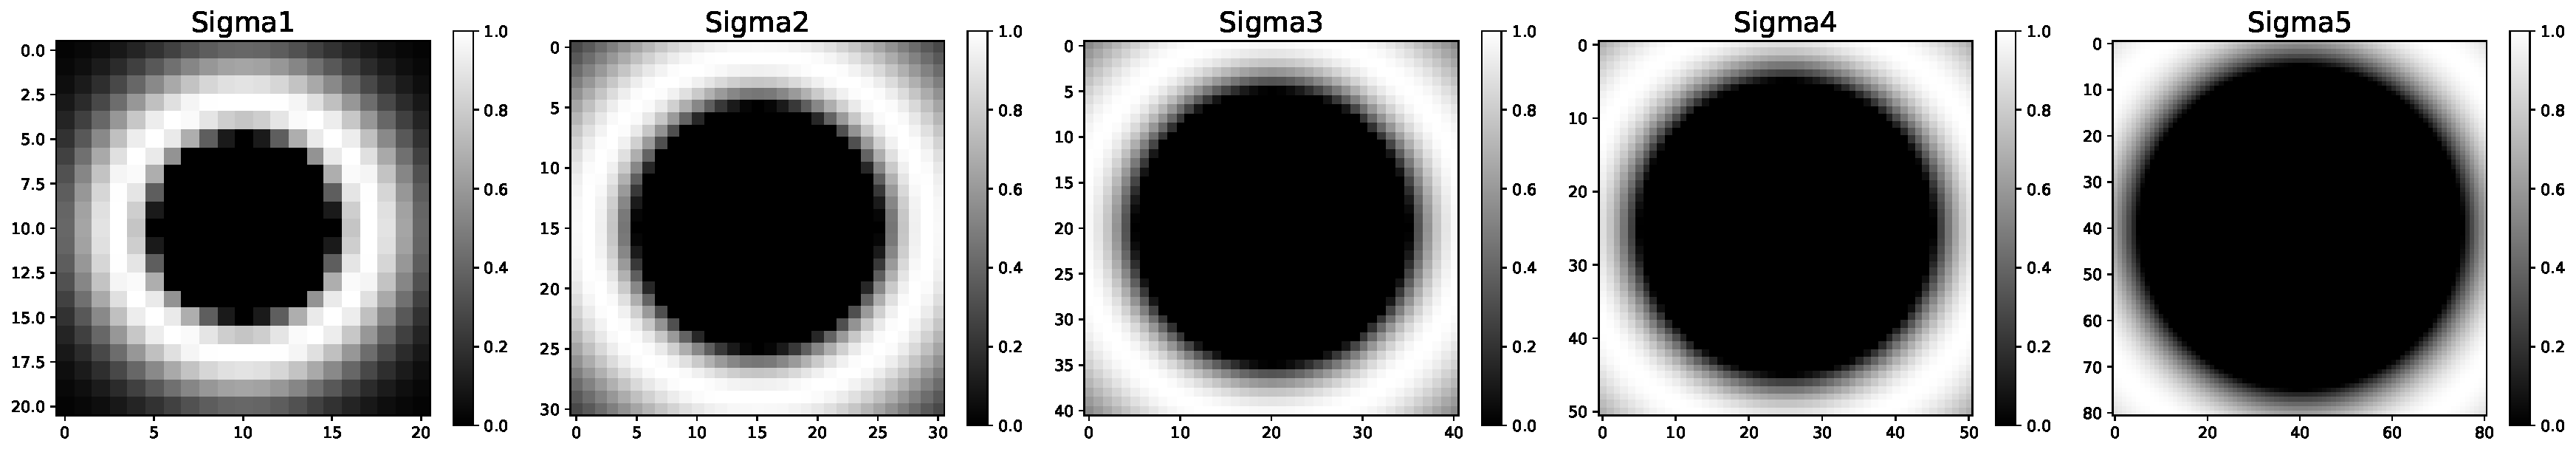
\includegraphics[width=1.0\linewidth]{Data/Solutions/question_2_7.pdf}
    \end{figure}
\end{solution}

\subsection{Visualize the blob detection results \mypoints{3.0}}
(See the Jupyter notebook) In this sub-part you will visualize the blob detection results. Copy the saved image from the Jupyter notebook here. 
\begin{solution}
\begin{figure}[H]
    \centering
    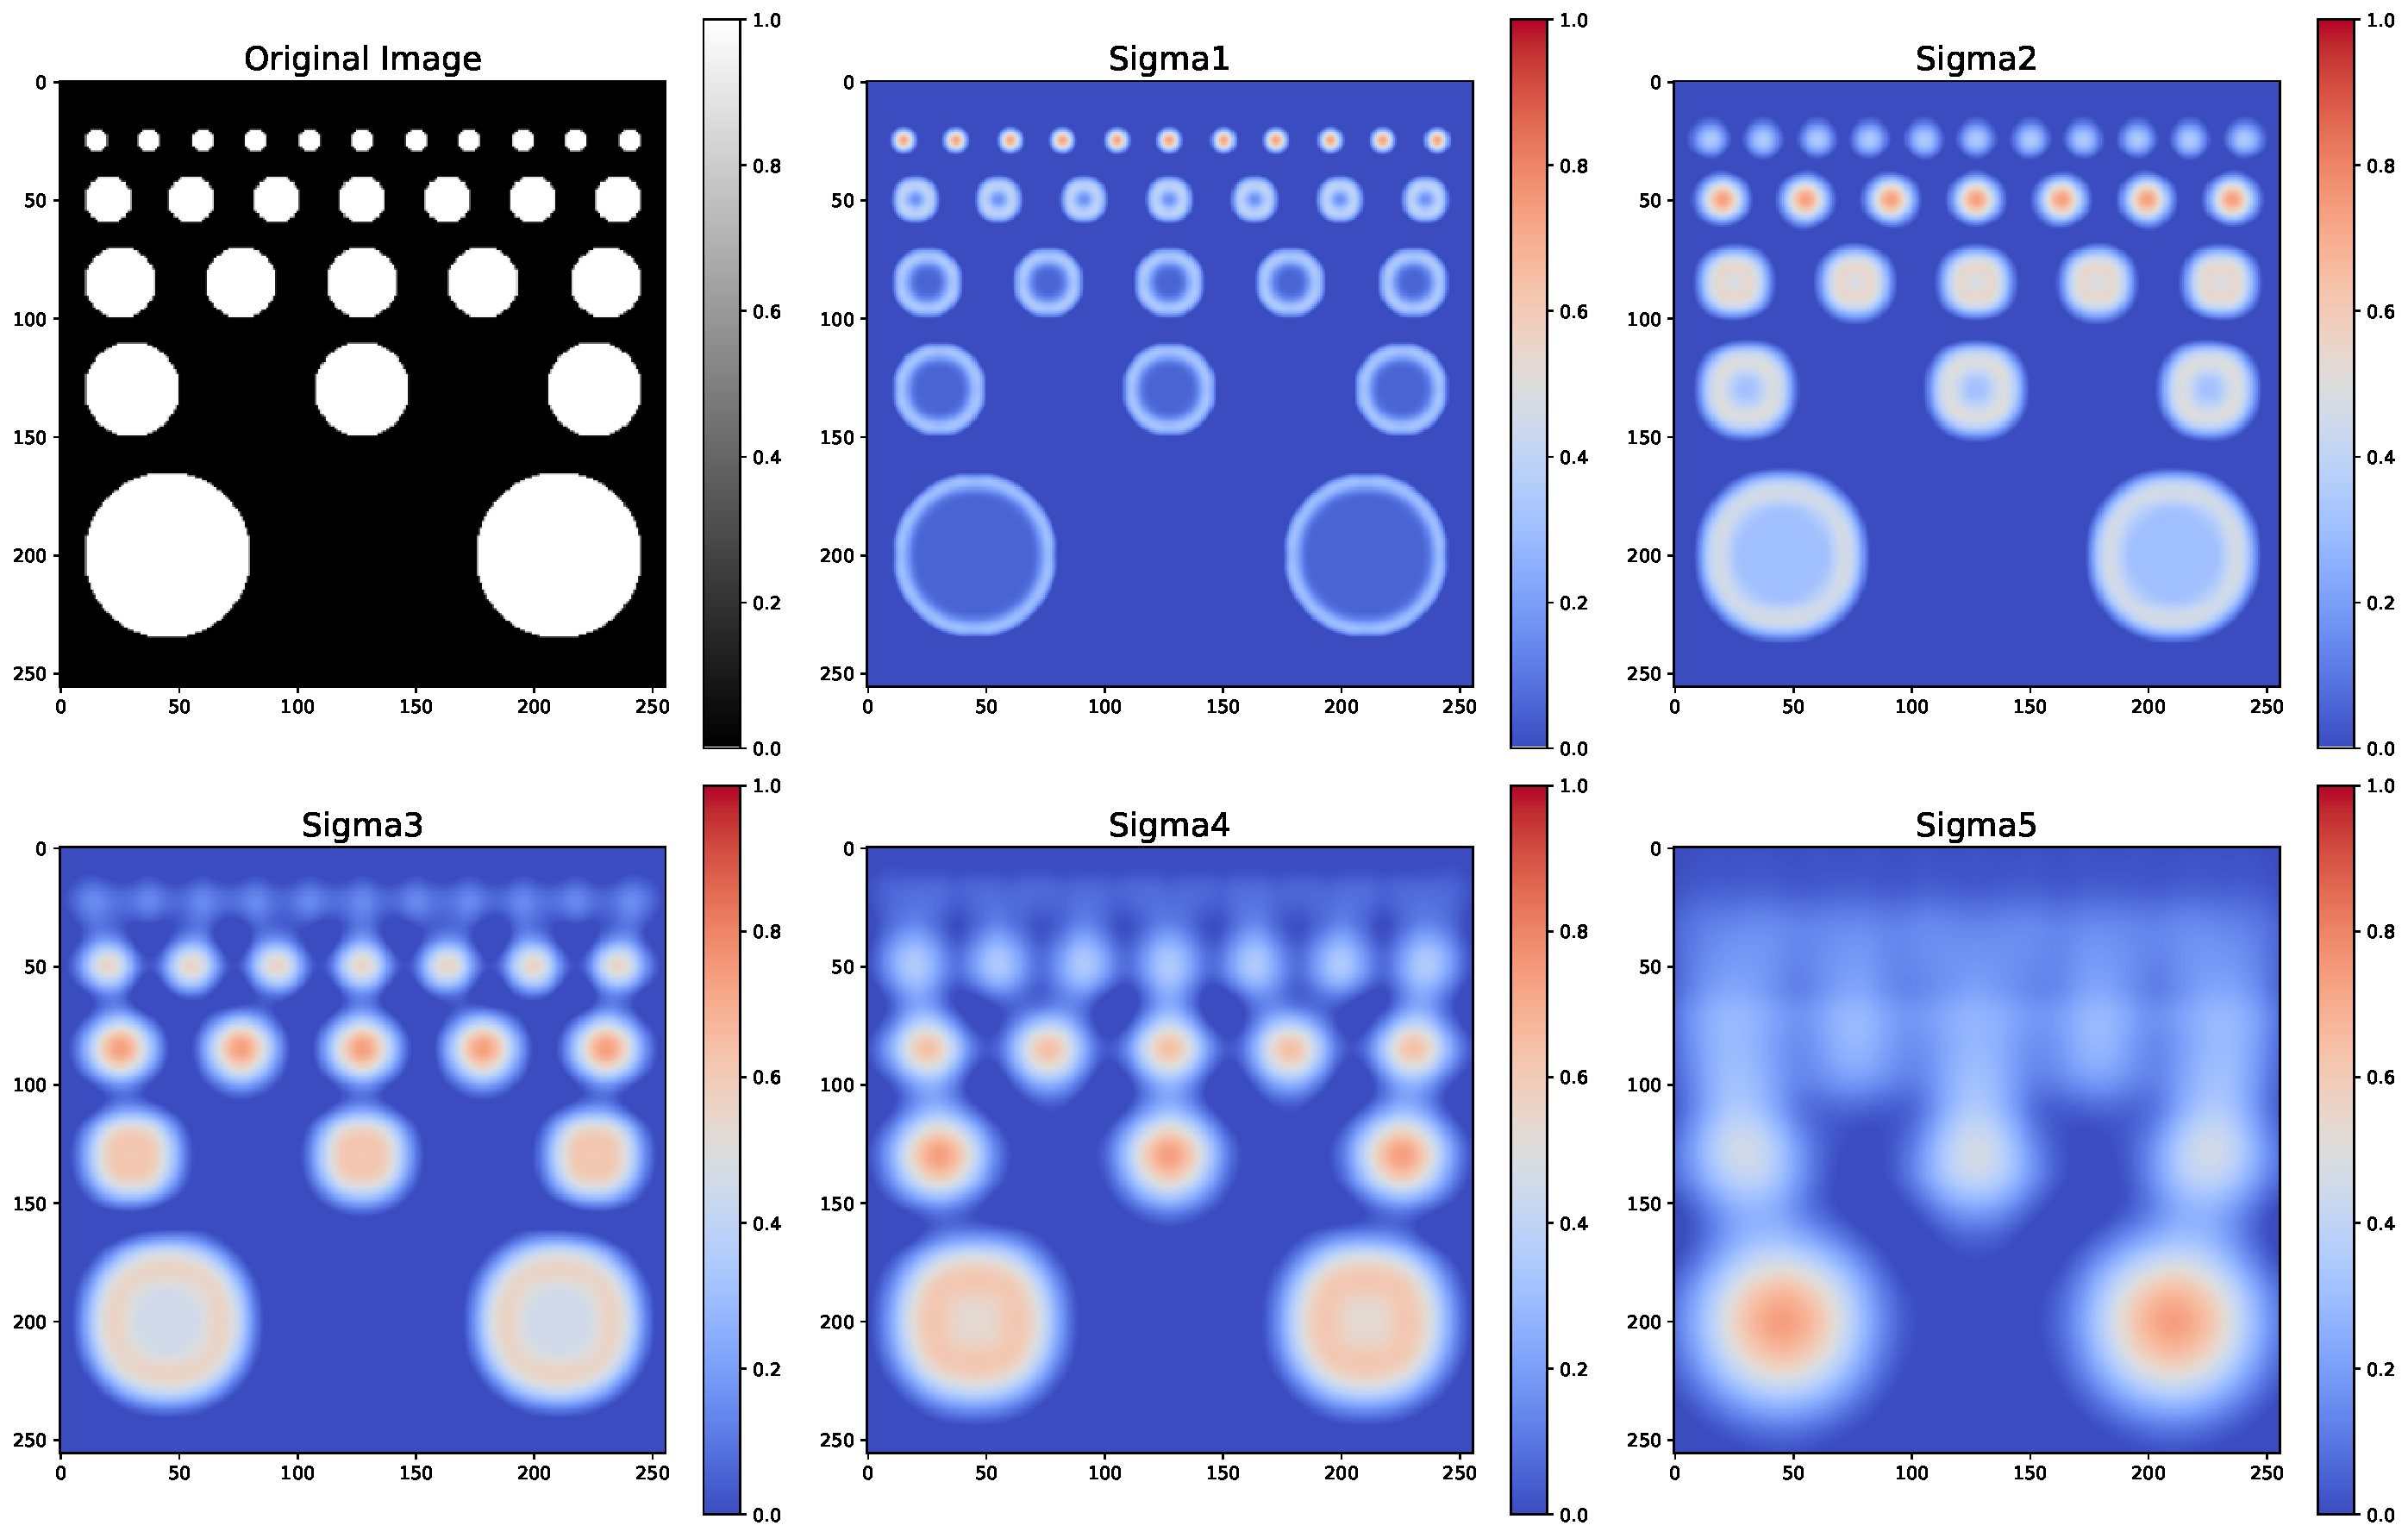
\includegraphics[width=1.0\linewidth]{Data/Solutions/question_2_8.pdf}
\end{figure}
\end{solution}

\newpage
\section{Corner Detection \mypoints{10.0}}

In this question, you will be implementing the Harris corner detector. As discussed in class, corners generally serve as useful features.

\subsection{Computing Image Gradients Using Sobel Filter \mypoints{1.0}}
(See the Jupyter notebook). In this sub-part, you will write a function that computes image gradients using the Sobel filter. Make sure that your code is within the bounding box.

\begin{solution}
\begin{minted}{python}
def compute_image_gradient(image: np.array):
    return conv2D(image, sobel_x), conv2D(image, sobel_y)
\end{minted}
\end{solution}

\subsection{Visualizing the Image Gradients \mypoints{1.0}}
(See the Jupyter notebook). In this sub-part, you will visualize the image gradients. Copy the saved image from the Jupyter notebook here.

\begin{solution}
\begin{figure}[H]
    \centering
    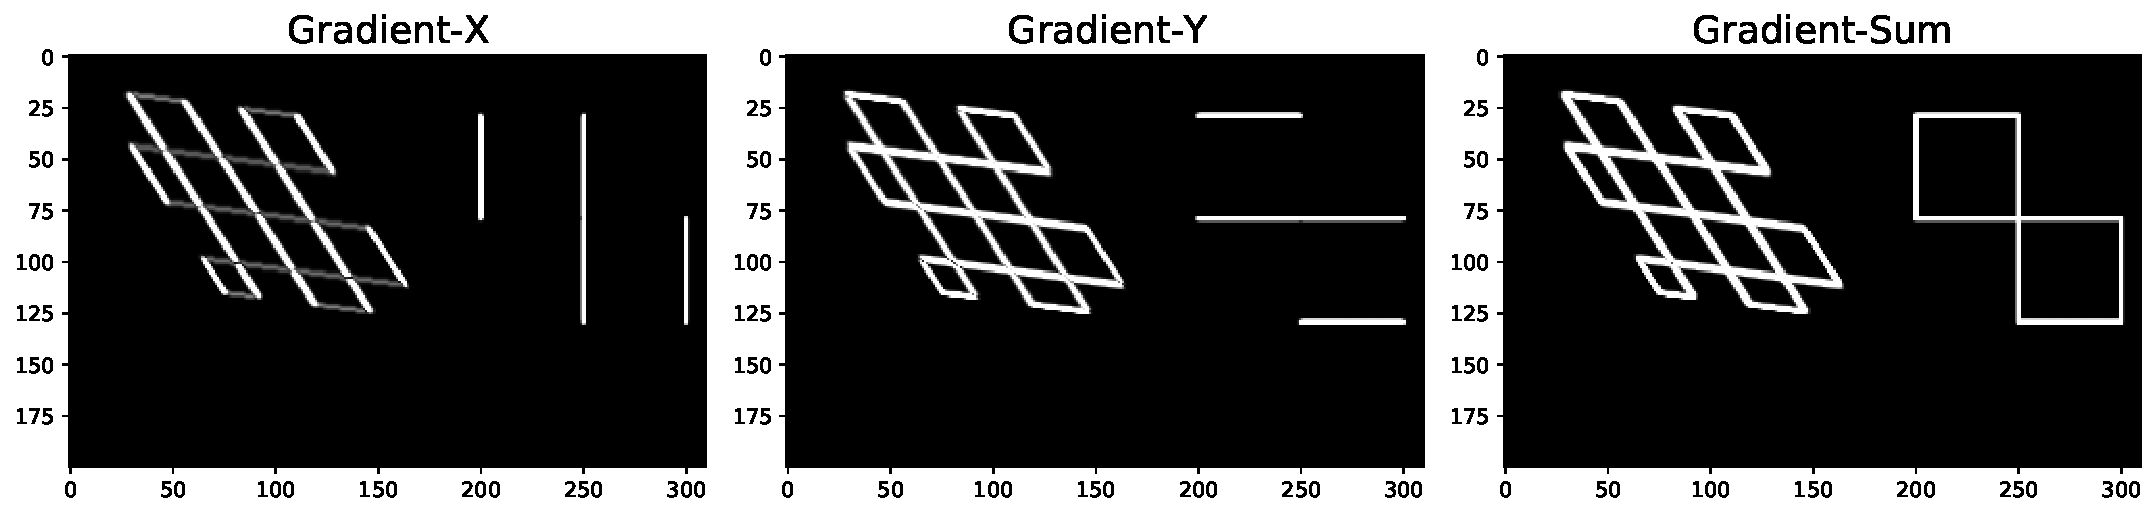
\includegraphics[width=\linewidth]{Data/Solutions/question_3_2.pdf}
\end{figure}
\end{solution}

\subsection{Computing the Covariance Matrix \mypoints{1.0}}
(See the Jupyter notebook). In this sub-part, you will write a function that computes the covariance matrix of the image gradients. Make sure that your code is within the bounding box.

\begin{solution}
\begin{minted}[breaklines]{python}
def grad_covariance(image: np.array, size: int):
    dx, dy = compute_image_gradient(image)
    Ixx, Ixy, Iyy = dx**2, dy*dx, dy**2
    i_xx, i_yy, i_xy = (conv2D(I, average_filter(size)) for I in (Ixx, Iyy, Ixy))
    return (i_xx, i_xy, i_yy)
\end{minted}
\end{solution}

\subsection{Harris Corner Response \mypoints{1.0}}
(See the Jupyter notebook). In this sub-part, you will write a function that computes the Harris response function. Make sure that your code is within the bounding box.

\begin{solution}
\begin{minted}[breaklines]{python}
def harris_response(image: np.array, k: float, size: int):
    i_xx, i_xy, i_yy = grad_covariance(image, size)
    ret = np.empty_like(image)
    for r in range(image.shape[0]):
        for c in range(image.shape[1]):
            a = np.array([[i_xx[r][c], i_xy[r][c]], [i_xy[r][c], i_yy[r][c]]])
            ret[r, c] = np.linalg.det(a) - k * (np.trace(a)) ** 2
    return ret
\end{minted}
\end{solution}

\subsection{Visualizing the Harris Corner Detector \mypoints{1.0}}
(See the Jupyter notebook). In this sub-part, you will visualize the Harris corner detections. Copy the saved image from the Jupyter notebook here.

\begin{solution}
\begin{figure}[H]
    \centering
    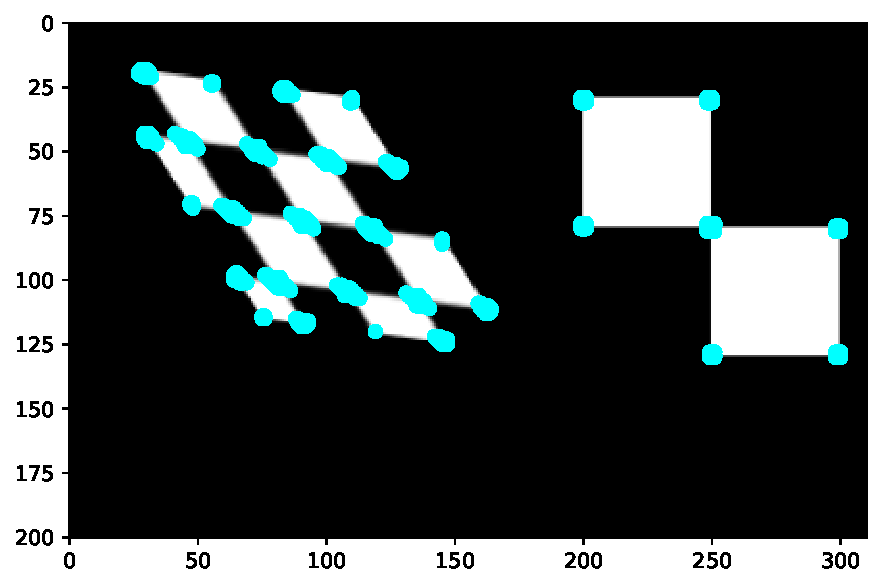
\includegraphics[width=\linewidth]{Data/Solutions/question_3_5.pdf}
\end{figure}
\end{solution}

\subsection{Thresholding the Harris Response \mypoints{1.0}}
To remove duplicate detections, you will write a function that applies non-maximum suppression to the Harris corner detections. To make writing this function easier, you will implement it in various parts.

(See the Jupyter notebook). In this sub-part, you will implement the first step of non-maximum suppression: thresholding the Harris response to obtain candidate corner detections. Make sure that your code is within the bounding box.

\begin{solution}
\begin{minted}[breaklines]{python}
def threshold_harris_response(harris_response: np.array, threshold: float):
    return np.argwhere(harris_response > threshold)
\end{minted}
\end{solution}

\subsection{Sorting Candidate Detections \mypoints{1.0}}
(See the Jupyter notebook). In this sub-part, you will sort the candidate detections by maximum Harris response value. Make sure that your code is within the bounding box.

\begin{solution}
\begin{minted}[breaklines]{python}
def sort_detections(candidate_detections: np.array, harris_response: np.array):
    sorted_detection_responses = np.argsort(-harris_response[candidate_detections[:,0], candidate_detections[:, 1]])
    return [candidate_detections[ind] for ind in sorted_detection_responses]
\end{minted}
\end{solution}

\subsection{Suppressing Non-max Detections \mypoints{1.0}}
(See the Jupyter notebook). In this sub-part, you will implement the final step of non-maximum suppression: removing corner detections that are not local maxima. Make sure that your code is within the bounding box.

\begin{solution}
\begin{minted}[breaklines]{python}
def local_max(sorted_detections: np.array, distance: float):
    valid_detections = []
    while sorted_detections:
        top = sorted_detections.pop(0)
        if not any(l2_distance(top, d) < distance for d in valid_detections):
            valid_detections.append(top)
    return np.asarray(valid_detections)
\end{minted}
\end{solution}

\subsection{Non-Maximum Suppression: Putting it all together \mypoints{1.0}}
(See the Jupyter notebook). In this sub-part, you will write a function that performs non-maximum suppression on the Harris corner response. Make sure that your code is within the bounding box.

\begin{solution}
\begin{minted}[breaklines]{python}
def non_max_suppression(harris_response: np.array, distance: float, threshold: float):
    t_responses = threshold_harris_response(harris_response, threshold)
    sorted_candidates = sort_detections(t_responses, harris_response)
    return local_max(sorted_candidates, distance)
\end{minted}
\end{solution}


\subsection{Visualizing Harris Corner Detections + Non-maximum Suppression \mypoints{1.0}}
(See the Jupyter notebook). In this sub-part, you will visualize the Harris corner detections after non-maximum suppression has been applied. Copy the saved image from the Jupyter notebook here. Duplicate corner detections should now be removed.

\begin{solution}
\begin{figure}[H]
    \centering
    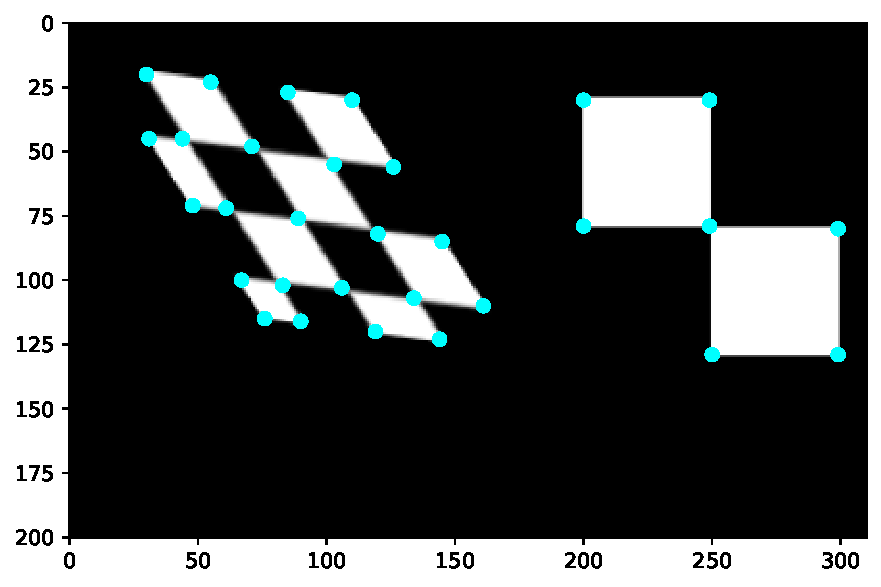
\includegraphics[width=\linewidth]{Data/Solutions/question_3_10.pdf}
\end{figure}
\end{solution}

\newpage
\section{2D Transformation \mypoints{10.0}}
In this question, you will be identifying different 2D transformations. You will be given a set of feature points $x$ and the corresponding transformed points $x'$. Given these two set of points, you have to identify the 2D transformation. For the first 5 sub-parts, there is only one transformation (translation, scaling, rotation, shearing). For the next parts, there may be more than one transformation.
While justifying your answer for each part you should also write the $3 \times 3$ transformation matrix $M$.

\subsection{Example 1 \mypoints{1.0}}
$x = \{(1,1), (2,1), (2,2), (1,2)\}$ and $x' = \{(2,2), (3,2), (3,3), (2,3)\}$. Identify the transformation and justify:
\begin{solution}
$
M = \begin{pmatrix}
1 & 0 & 1\\
0 & 1 & 1\\
0 & 0 & 1
\end{pmatrix}
$
\\\\
We have a translation by $(1, 1)$
\end{solution}

\subsection{Example 2 \mypoints{1.0}}
$x = \{(1,1), (2,1), (2,2), (1,2)\}$ and $x' = \{(0,\sqrt{2}), (\sqrt{2}-\frac{1}{\sqrt{2}},\sqrt{2}+\frac{1}{\sqrt{2}}), (0,2\sqrt{2}), (\frac{1}{\sqrt{2}}-\sqrt{2},\sqrt{2}+\frac{1}{\sqrt{2}})\}$. Identify the transformation and justify:
\begin{solution}
$
M = \begin{pmatrix}
1/\sqrt{2} & -1/\sqrt{2} & 0\\
1/\sqrt{2} & 1/\sqrt{2} & 0\\
0 & 0 & 1
\end{pmatrix}
$
\\\\
We have a rotation by $\frac{\pi}{4}$
\end{solution}

\subsection{Example 3 \mypoints{1.0}}
$x = \{(1,1), (2,1), (2,2), (1,2)\}$ and $x' = \{(-1,1), (-1,2), (-2,2), (-2,1)\}$. Identify the transformation and justify:
\begin{solution}
$
M = \begin{pmatrix}
0 & -1 & 0\\
1 & 0 & 0\\
0 & 0 & 1
\end{pmatrix}
$
\\\\
We have a rotation by $\frac{\pi}{2}$
\end{solution}

\subsection{Example 4 \mypoints{1.0}}
$x = \{(1,1), (2,1), (2,2), (1,2)\}$ and $x' = \{(3,5), (6,5), (6,10), (3,10)\}$. Identify the transformation and justify:
\begin{solution}
$
M = \begin{pmatrix}
3 & 0 & 0\\
0 & 5 & 0\\
0 & 0 & 1
\end{pmatrix}
$
\\\\
We have a scaling by (3, 5) in the (x, y) axes respectively
\end{solution}

\subsection{Example 5 \mypoints{1.0}}
$x = \{(1,1), (2,1), (2,2), (1,2)\}$ and $x' = \{(4,6), (5,11), (8,12), (7,7)\}$. Identify the transformation and justify:
\begin{solution}
$
M = \begin{pmatrix}
1 & 3 & 0\\
5 & 1 & 0\\
0 & 0 & 1
\end{pmatrix}
$
\\\\
We have a shearing by (5, 3) in the (x, y) axes respectively
\end{solution}

\subsection{Example 6 \mypoints{1.0}}
$x = \{(1,1), (2,1), (2,2), (1,2)\}$ and $x' = \{(0,2), (0,3), (-1,3), (-1,2)\}$. Identify the two transformations and their order and justify:

\begin{solution}
$
M = \begin{pmatrix}
0 & -1 & 1\\
1 & 0 & 1\\
0 & 0 & 1
\end{pmatrix}
$
\\\\
First we have a rotation by -$\frac{\pi}{2}$ then a translation by (+1,+1).
\end{solution}

\subsection{Example 7 \mypoints{1.0}}
$x = \{(1,1), (2,1), (2,2), (1,2)\}$ and $x' = \{(-2,2), (-2,3), (-3,3), (-3,2)\}$. Identify the two transformations and their order and justify:

\begin{solution}
$
M = \begin{pmatrix}
0 & -1 & -1\\
1 & 0 & 1\\
0 & 0 & 1
\end{pmatrix}
$
\\\\
First we have a rotation by $-\frac{\pi}{2}$ and then a translation by (-1,+1).
\end{solution}

\subsection{Example 8 \mypoints{1.0}}
$x = \{(1,1), (2,1), (2,2), (1,2)\}$ and $x' = \{(4, 6), (7,6), (7,11), (4,11)\}$. Identify the two transformations and their order and justify:

\begin{solution}
$
M = \begin{pmatrix}
3 & 0 & 1\\
0 & 5 & 1\\
0 & 0 & 1
\end{pmatrix}
$
\\\\
First we have a scaling in the x-direction by a factor of 3 and scaling in the y-direction by a factor of 5. Then we have a translation by (+1,+1).
\end{solution}

\subsection{Example 9 \mypoints{1.0}}
$x = \{(1,1), (2,1), (2,2), (1,2)\}$ and $x' = \{(-5,3), (-5,6), (-10,6), (-10,3)\}$. Identify the two transformations and their order and justify:

\begin{solution}
$
M = \begin{pmatrix}
0 & -5 & 0\\
3 & 0 & 0\\
0 & 0 & 1
\end{pmatrix}
$
\\\\
First we have a rotation by $\frac{\pi}{2}$ and then a scaling by (5, 3) for the (x, y) axes respectively.
\end{solution}

\subsection{Example 10 \mypoints{1.0}}
$x = \{(1,1), (2,1), (2,2), (1,2)\}$ and $x' = \{(-6,4), (-11,5), (-12,8), (-7,7)\}$. Identify the two transformations and their order and justify:

\begin{solution}
$
M = \begin{pmatrix}
-5 & -1 & 0\\
1 & 3 & 0\\
0 & 0 & 1
\end{pmatrix}
$
\\\\
First we have a shearing by (5, 3) in the (x, y) axes respectively, and then we have a rotation by $\frac{\pi}{2}$.
\end{solution}

\newpage 

\section{Interview Question \mypoints{5.0}}

Object detection is a technique which allows computers to identify and localize objects in images/videos. Let us consider that we have an object detection system that finds cars in a given image. The object detection system will propose some candidates for the object. You can see multiple candidates for the car in Figure \ref{interview} (left), and the final bounding box for the car in Figure \ref{interview} (right). Each bounding box has a score which measures the likelihood of finding a car. Given the set of bounding boxes with their locations and their scores, propose a method for generating just one bounding box per object. Use one of the algorithms that has been covered in the class or even this homework.

\emph{Hint}: One metric for measuring whether different bounding boxes are in the same local ``neighborhood" is intersection over union (IoU), which is defined as follows:
\begin{equation*}
\text{IoU}(\text{box1}, \text{box2}) = \frac{\text{Area of intersection of box1 and box2}}{\text{Area of union of box1 and box2}}.
\end{equation*}

\begin{figure}[H]
    \centering
    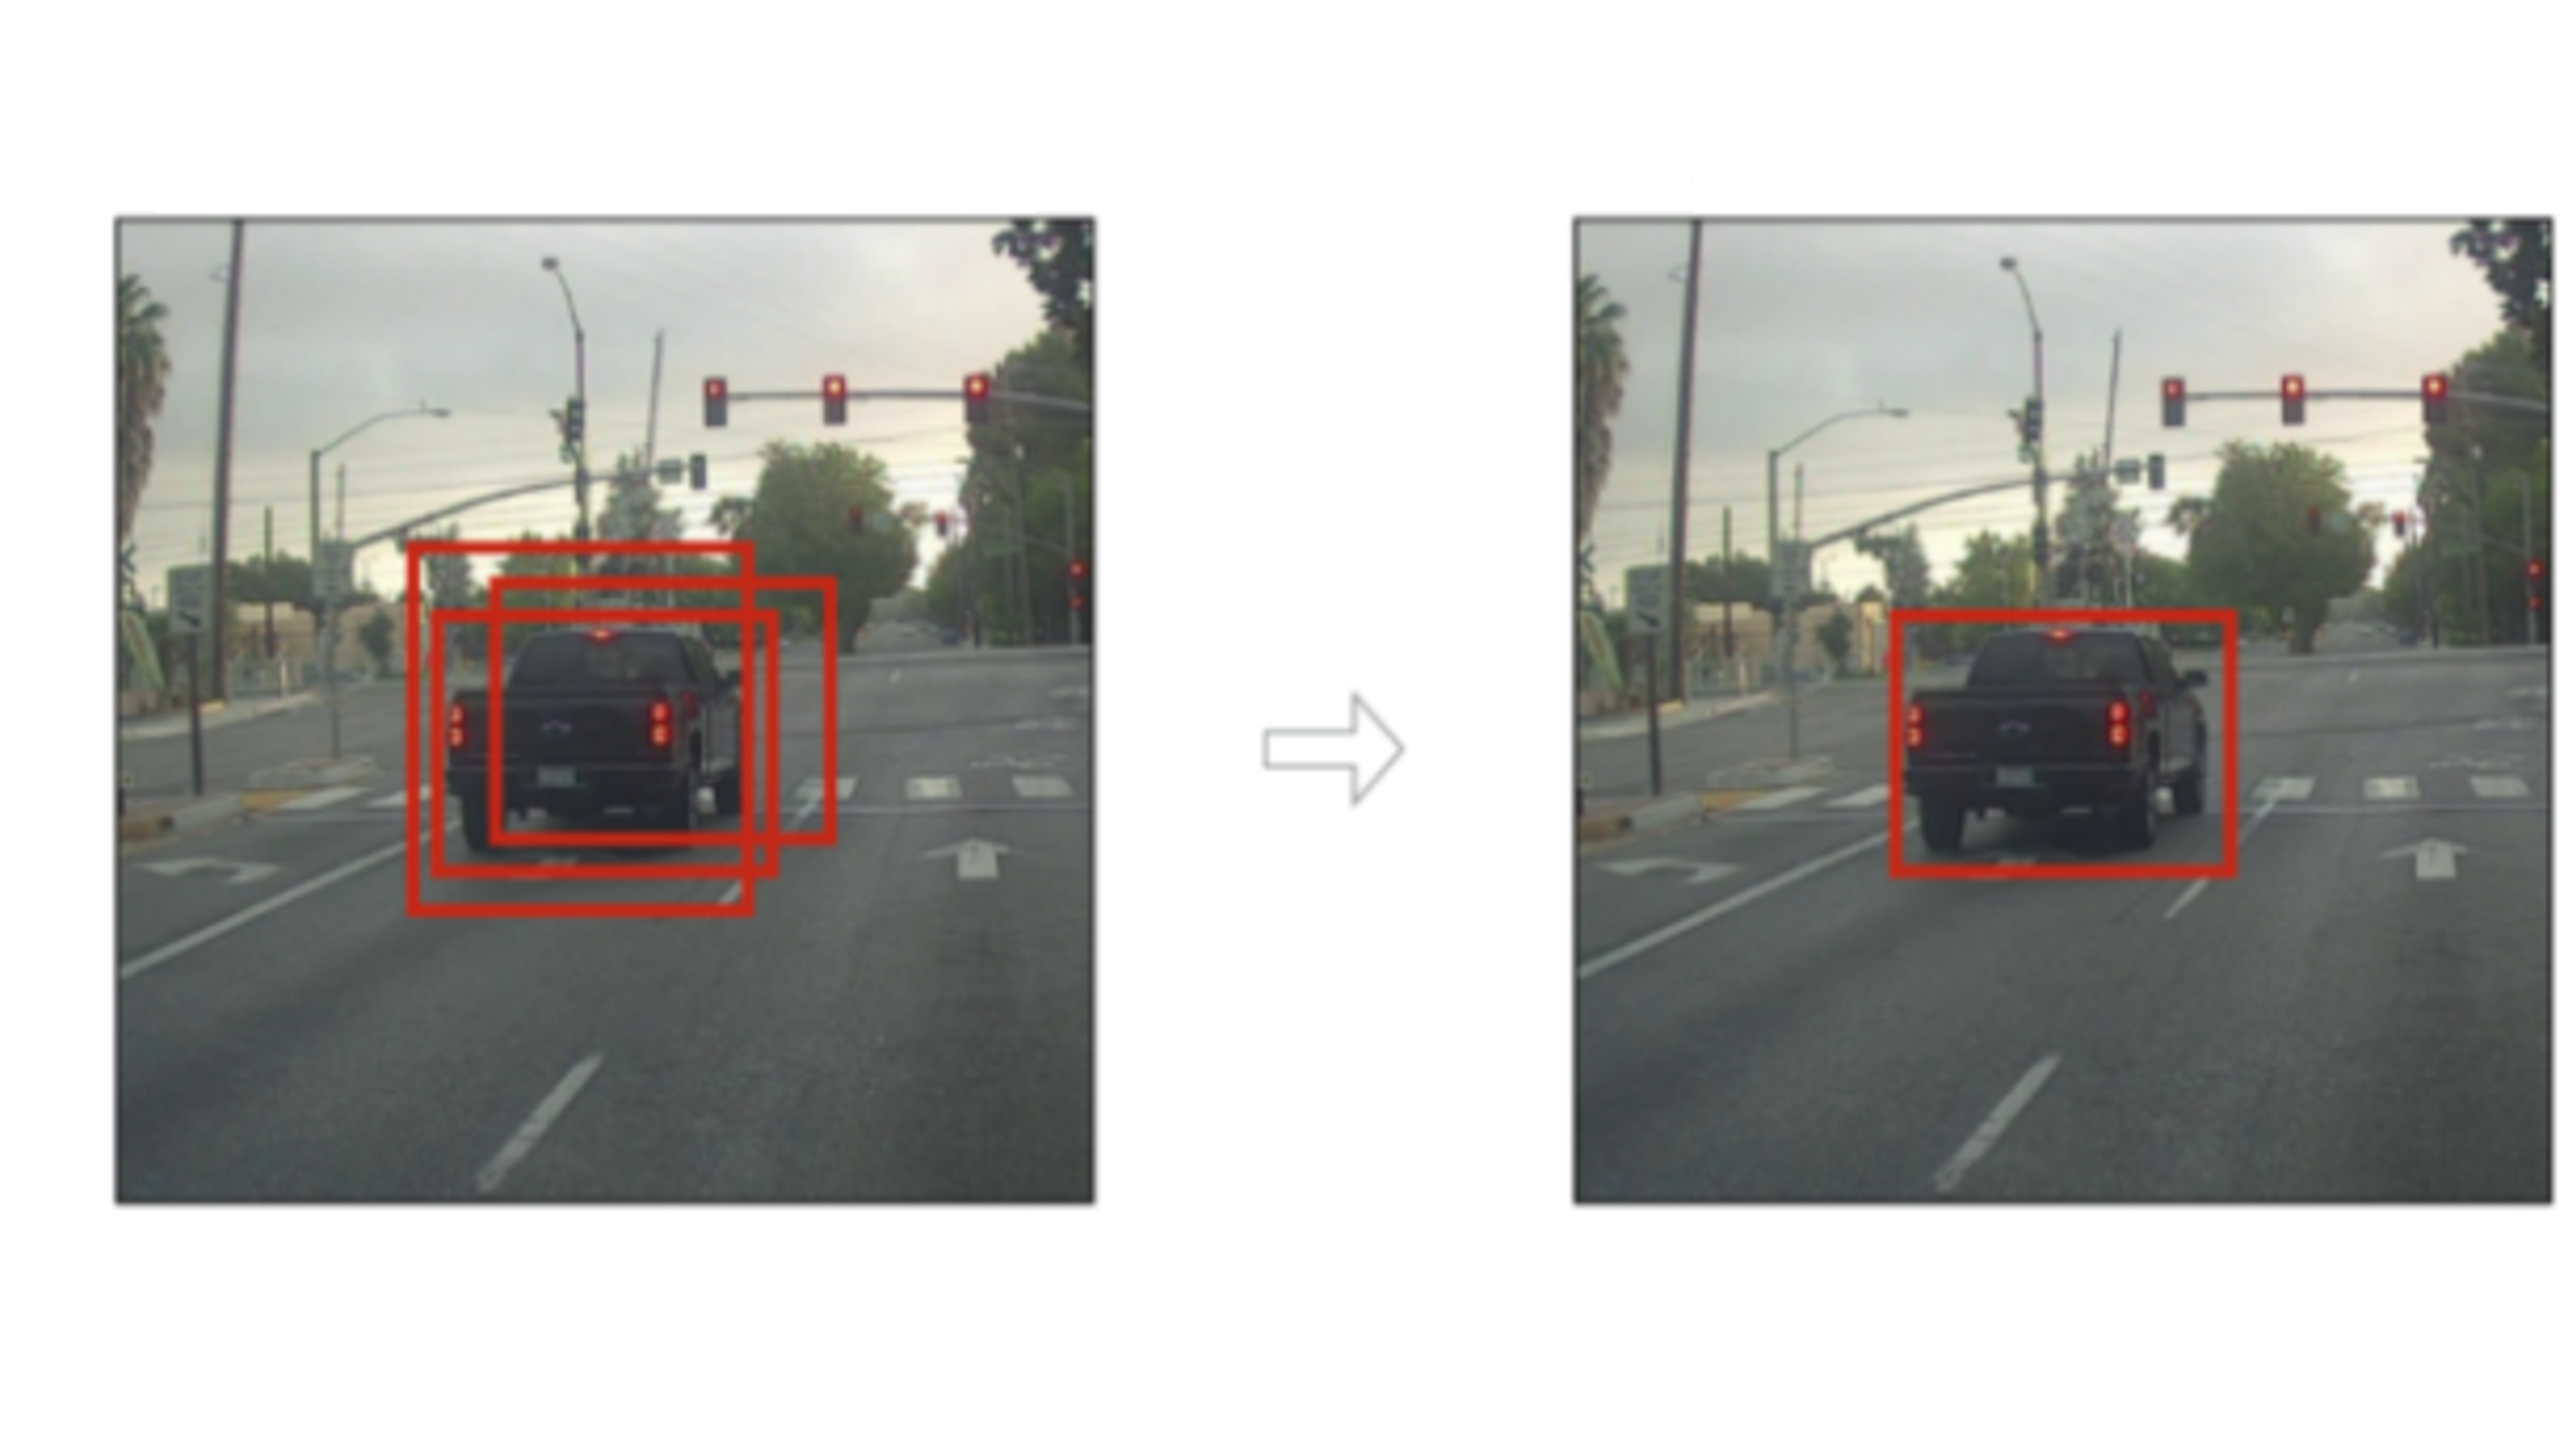
\includegraphics[width=\linewidth]{Images/interview.pdf}
\caption{(Left) The object detection system identifies many candidates for the location of the car. For each candidate, there is a score which measures how likely it is to find a car in that bounding box. You can see that there are multiple red boxes, where each box will have a score between 0-1. (Right) The final bounding box for the car.}
\label{interview}
\end{figure}

\begin{solution}
We can use the same local non-max suppression that we did for the Harris Corner Detector. In this case, we will use the "intersection over union" (IoU) instead of our l2\_distance as our metric for "distance" between boxes. A high IoU implies a significant amount of overlap between two bounding boxes and therefore a higher likelihood that the two boxes represent the same feature of the image. We can then use the score given by the bounding box to sort our detections (bounding boxes).

An example implementation in python might be similar to the following:

\begin{minted}[breaklines]{python}
def prune_boxes(bounding_boxes: np.array, iou_threshold: float):
    pruned_boxes = []
    box_queue = sorted(bounding_boxes, key=lambda x: x.score)
    while box_queue:
        box = box_queue.pop(0)
        if not any(IoU(box, b) < iou_threshold for b in pruned_boxes):
            pruned_boxes.append(box)
    return np.asarray(pruned_boxes)
    \end{minted}
\end{solution}


\end{document}